\documentclass[12pt, a4paper]{article}
\usepackage[margin=1.25in]{geometry}
\usepackage{graphicx}
\usepackage{amsmath}
\usepackage{float}
\usepackage{listings}
\usepackage{caption}
\usepackage[shortlabels]{enumitem}


\setlength\parindent{0pt}
\newcommand{\code}{\lstinline[basicstyle=\small]}
\lstset{
    language=Python,
    basicstyle=\scriptsize
}


\title{EE2703: Applied Programming Lab \\ \Large Assignment 5: Laplace Equation}
\author{Soham Roy \\ \normalsize EE20B130}
\date{\today}
\begin{document}

\maketitle % Insert the title, author and date


\bigskip
\section{Introduction}
The currents in a resistor will be evaluated. The currents depend on the shape of the resistor.
The part of the resistor likely to get hottest is also visualised. \\
\medskip

A wire is soldered to the middle of a copper plate and its voltage is held at 1 Volt. One side of the plate is
grounded, while the remaining are floating. The plate is 1 cm by 1 cm in size.

By the conductivity:
\begin{equation*}
    \vec{j} = \sigma \vec{E}
\end{equation*}

As the Electric field is the gradient of the potential:
\begin{equation*}
    \vec{E} = - \nabla \phi
\end{equation*}

Continuity of charge yields:
\begin{equation*}
    \nabla \cdot \vec{j} = - \frac{\partial \rho}{\partial t}
\end{equation*}

Combining these equations:
\begin{equation*}
    \nabla \cdot (- \sigma \nabla \phi) = - \frac{\partial \rho}{\partial t}
\end{equation*}

Assuming that the resistor consists of a material of constant conductivity:
\begin{equation*}
    \nabla^2 \phi = \frac{1}{\sigma} \frac{\partial \rho}{\partial t}
\end{equation*}

For DC currents the RHS is zero, thus:
\begin{equation*}
    \nabla^2 \phi = 0
\end{equation*}



\section{Subquestions}
\subsection{Import the Libraries}
The following libraries have been imported:
\begin{lstlisting}
    import sys
    import argparse
    import numpy as np
    import matplotlib.pyplot as plt

    from scipy.linalg import lstsq
\end{lstlisting}
\code{sys} and \code{argparse} are used to parse the command line arguments. \\
\code{numpy} and \code{matplotlib} are used for numerical computation and plotting. \\
\code{scipy.linalg.lstsq} is used to extract best fits for the linear system.


\subsection{Define the Parameters}
The following parameters have been defined:
\begin{lstlisting}
    Nx, Ny, radius, Niter = parse_cmdline_args()  # define the parameters
\end{lstlisting}
Here, \code{parse_cmdline_args()} is a function that parses the command line arguments and returns
the parameters as either user inputs or their default values. It employs the following code:
\begin{lstlisting}
    try:  # try converting directly to values
        return [
            int(sys.argv[1]) if len(sys.argv) >= 2 else 25,
            int(sys.argv[2]) if len(sys.argv) >= 3 else 25,
            int(sys.argv[3]) if len(sys.argv) >= 4 else 8,
            int(sys.argv[4]) if len(sys.argv) >= 5 else 1500,
        ]
    except ValueError:  # otherwise, parse keyword arguments
        parser = argparse.ArgumentParser(description="Resistor simulation")

        parser.add_argument(
            "-x", "--Nx", type=int, default=25, help="size along x axis"
        )
        parser.add_argument(
            "-y", "--Ny", type=int, default=25, help="size along y axis"
        )
        parser.add_argument(
            "-r", "--radius", type=int, default=8, help="radius of central lead"
        )
        parser.add_argument(
            "-n", "--Niter", type=int, default=1500, help="number of iterations"
        )

        args = parser.parse_args()

        return args.Nx, args.Ny, args.radius, args.Niter

\end{lstlisting}
\pagebreak


\subsection{Initialize the Potential Array} \label{sec:contour}
The potential array $\phi$ has been generated by:
\begin{lstlisting}
    phi = np.zeros((Ny, Nx))  # allocate the potential array
    X, Y = np.meshgrid(np.linspace(-0.5, 0.5, Nx), np.linspace(-0.5, 0.5, Ny))

    # scaled radius = 0.35 for default args, 5% margin for floating point errors
    ii = np.where(X ** 2 + Y ** 2 <= (1.05 * radius / (min(Nx, Ny) - 1)) ** 2)
    phi[ii] = 1.0  # initialize the potential array   
\end{lstlisting}
The \code{contour_plot()} function obtains a contour plot of the potential,
with the nodes in the $V=1$ region marked red, by the following:
\begin{lstlisting}
    plt.clabel(plt.contour(X, Y, phi))
    plt.scatter(X[0, ii[1]], Y[ii[0], 0], color="r", label="$V=1$")
\end{lstlisting}
\begin{figure}[H]
    \centering
    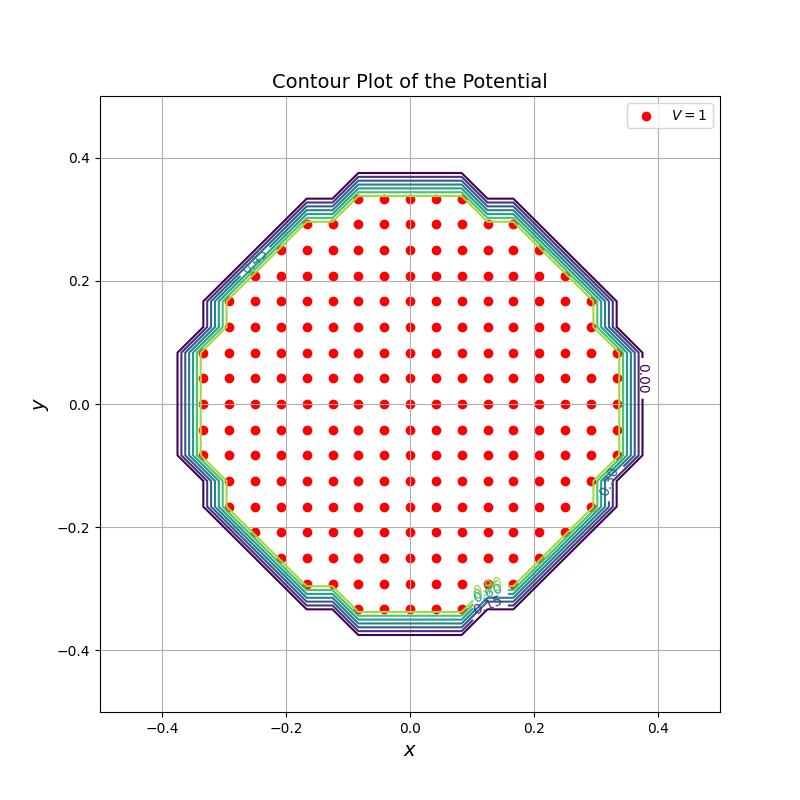
\includegraphics[scale=0.6]{3.png}
\end{figure}


\subsection{Perform the Iterations}
The \code{iterate()} function realizes the following logic:
\begin{lstlisting}
    for k in range(Niter)
        save copy of phi
        update phi array
        assert boundaries
        errors[k]=(abs(phi-oldphi)).max();
    #end
\end{lstlisting}
\pagebreak

Through this loop:
\begin{lstlisting}
    for k in range(Niter):
        oldphi = phi.copy()

        # updating the potential
        phi[1:-1, 1:-1] = (  # update interior points to average of neighbors
            phi[1:-1, :-2] + phi[1:-1, 2:] + phi[:-2, 1:-1] + phi[2:, 1:-1]
        ) / 4

        # boundary conditions
        phi[1:-1, 0] = phi[1:-1, 1]  # left
        phi[1:-1, -1] = phi[1:-1, -2]  # right
        phi[-1, :] = phi[-2, :]  # top
        phi[ii] = 1.0  # central area corresponding to electrodes to 1

        errors[k] = np.max(np.abs(phi - oldphi))
\end{lstlisting}
Subsections \ref{sec:updating} and \ref{sec:boundaries} explain the updating of the potential
and the boundary conditions respectively.


\subsection{Updating the Potential} \label{sec:updating}
The potential is updated according to the following equation:
\begin{equation*}
    \phi_{i,j} = \frac{\phi_{i-1,j} + \phi_{i+1,j} + \phi_{i,j-1} + \phi_{i,j+1}}{4}
\end{equation*}
This is accomplished by the following code:
\begin{lstlisting}
    phi[1:-1, 1:-1] = (  # update interior points to average of neighbors
        phi[1:-1, :-2] + phi[1:-1, 2:] + phi[:-2, 1:-1] + phi[2:, 1:-1]
    ) / 4
\end{lstlisting}


\subsection{Boundary Conditions} \label{sec:boundaries}
The boundary condition at the left boundary, for example, is:
\begin{equation*}
    \frac{\partial \phi}{\partial x} = 0
\end{equation*}
This is accomplished by the following code:
\begin{lstlisting}
    phi[1:-1, 0] = phi[1:-1, 1]  # left
    phi[1:-1, -1] = phi[1:-1, -2]  # right
    phi[-1, :] = phi[-2, :]  # top
    phi[ii] = 1.0  # central area corresponding to electrodes to 1
\end{lstlisting}
The potential of the nodes corresponding to the electrode region has been ensured to be $1$.
\pagebreak


\subsection{Graph the Results}
The \code{plot_errors()} function plots the errors vs iteration number:
\begin{figure}[H]
    \centering
    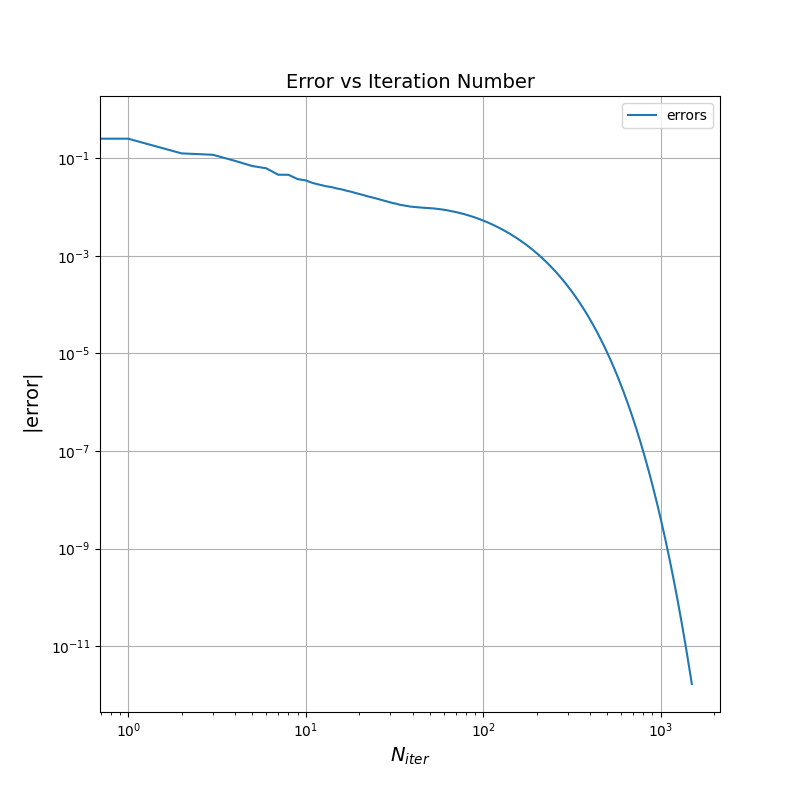
\includegraphics[scale=0.4]{7a.png}
    \caption*{log-log scale}
\end{figure}
\begin{figure}[H]
    \centering
    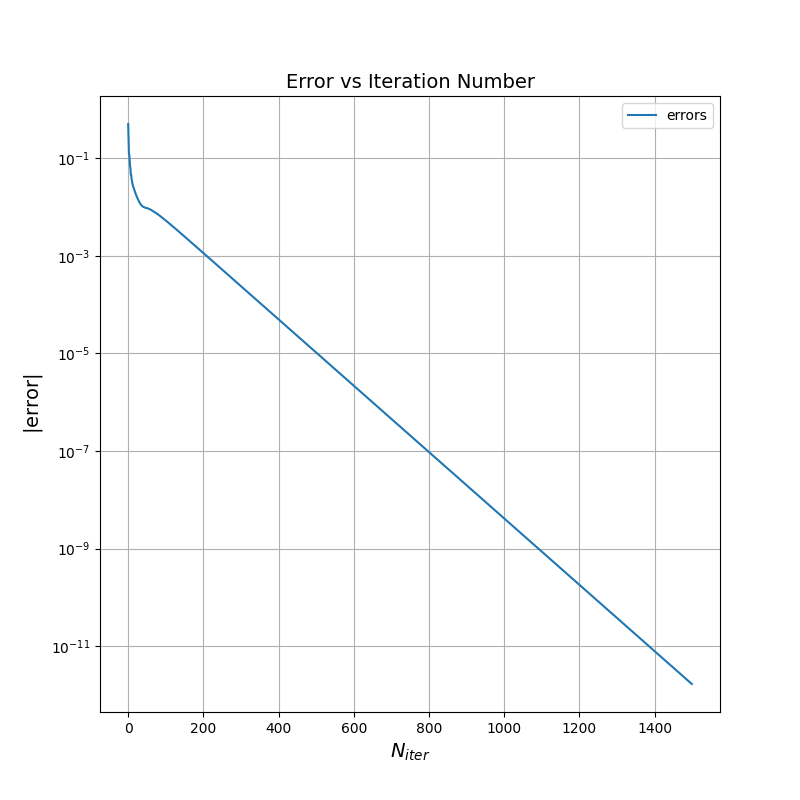
\includegraphics[scale=0.4]{7b.png}
    \caption*{semilog scale}
\end{figure}
\pagebreak

To see individual data points, every 50\textsuperscript{th} point has been plotted:
\begin{figure}[H]
    \centering
    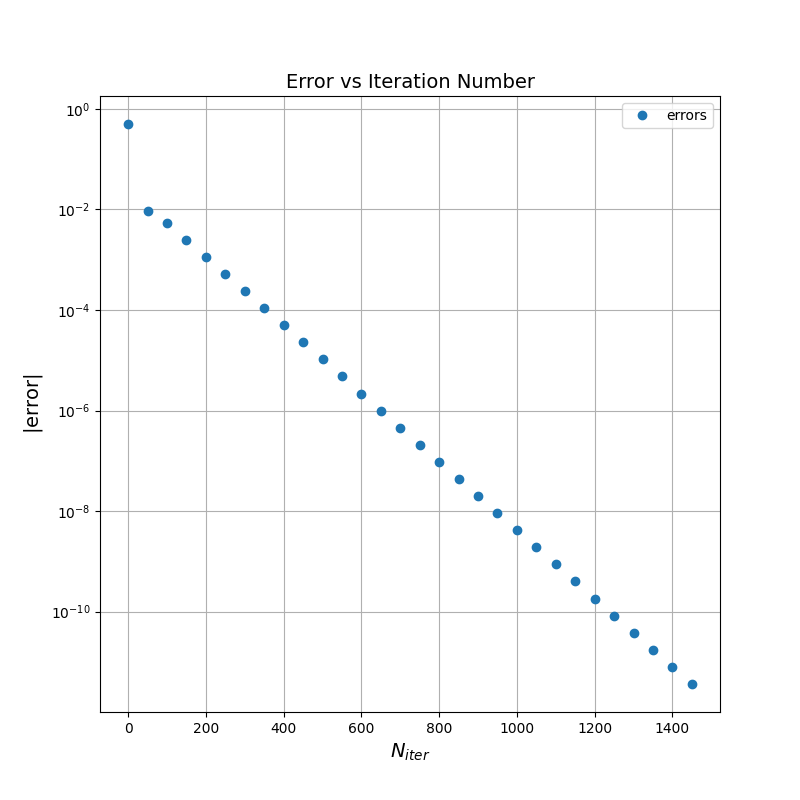
\includegraphics[scale=0.4]{7c.png}
\end{figure}

The data may be fit to an exponential, especially for larger iteration numbers (i.e. beyond 500):
\begin{equation*}
    y = Ae^{Bx} \implies \log y = \log A + Bx
\end{equation*}
The code used for this is:
\begin{lstlisting}
    fit1 = lstsq(np.c_[np.ones(len(errors)), n], np.log(errors))[0]
    fit2 = lstsq(np.c_[np.ones(len(errors)), n][500:], np.log(errors)[500:])[0]

    plt.semilogy(np.exp(fit1[0] + fit1[1] * n), "r", lw=3, label="fit1")
    plt.semilogy(np.exp(fit2[0] + fit2[1] * n), "g", label="fit2")
\end{lstlisting}
Where \code{n} is defined as \code{np.arange(len(errors))}.

\begin{figure}[H]
    \centering
    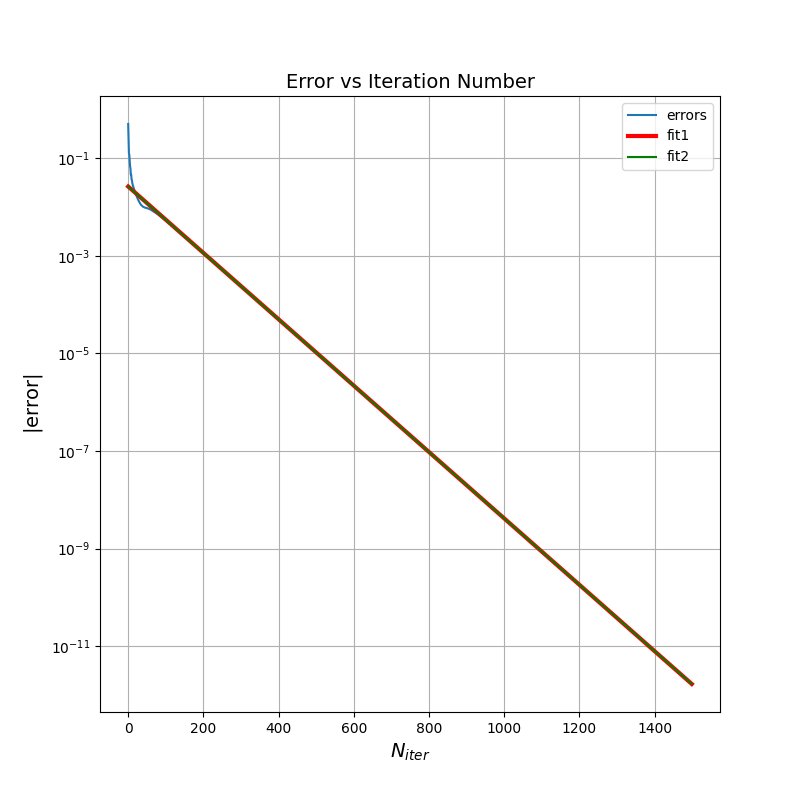
\includegraphics[scale=0.4]{7d.png}
\end{figure}


\subsection{Surface Plot of Potential}
The \code{surface_plot()} generates the surface plot by the following code:
\begin{lstlisting}
    ax = plt.figure(figsize=(8, 8)).add_subplot(projection="3d")  # new way
    plt.colorbar(ax.plot_surface(X, Y, phi, rstride=1, cstride=1, cmap=cm.jet))
\end{lstlisting}
\begin{figure}[H]
    \centering
    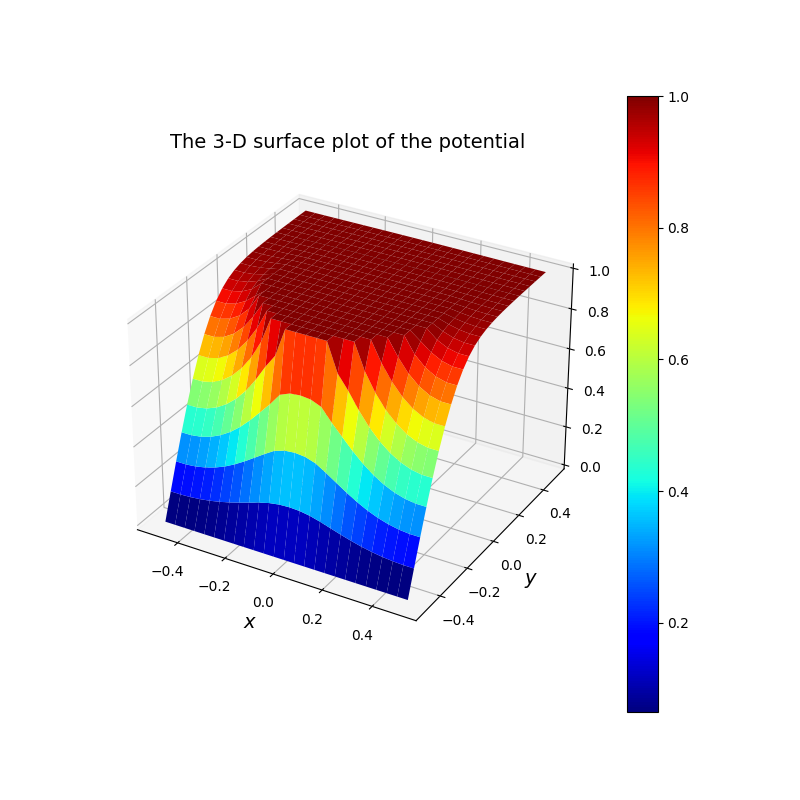
\includegraphics[scale=0.425]{8.png}
\end{figure}


\subsection{Contour Plot of Potential}
The same \code{contour_plot()} function from Subsection \ref{sec:contour} has been used:
\begin{figure}[H]
    \centering
    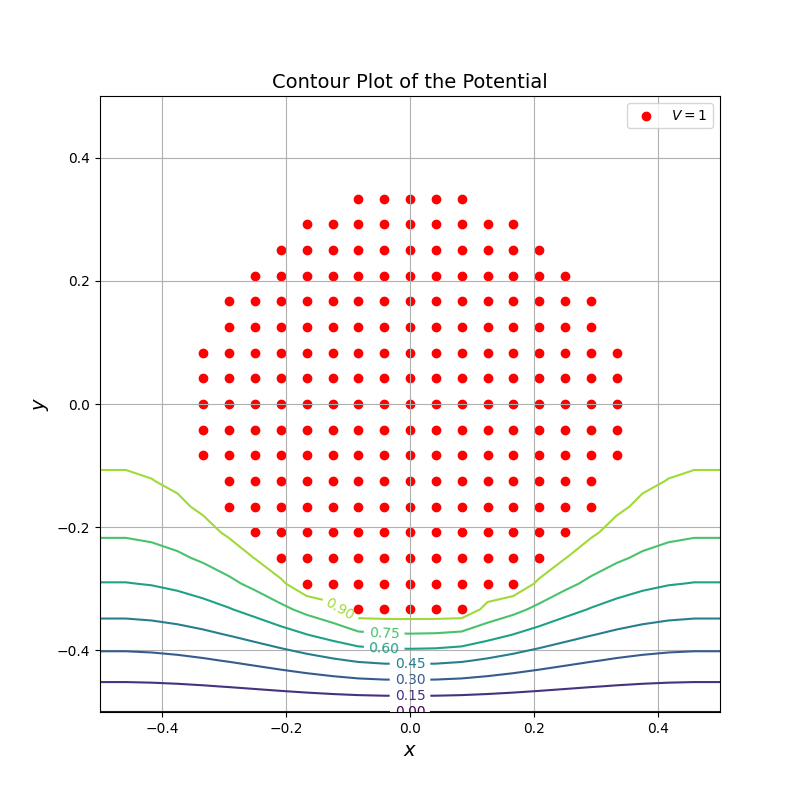
\includegraphics[scale=0.425]{9.png}
\end{figure}


\subsection{Vector Plot of Currents}
The currents are given by the following equations:
\begin{align*}
    J_{x,ij} & = \frac{1}{2} (\phi_{i,j-1} - \phi_{i,j+1}) \\
    J_{y,ij} & = \frac{1}{2} (\phi_{i-1,j} - \phi_{i+1,j})
\end{align*}

The \code{plot_currents()} function implements these equations as:
\begin{lstlisting}
    Jx, Jy = np.zeros_like(phi), np.zeros_like(phi)
    Jx[:, 1:-1] = (phi[:, :-2] - phi[:, 2:]) / 2
    Jy[1:-1, :] = (phi[:-2, :] - phi[2:, :]) / 2
\end{lstlisting}

These matrices are subsequently plotted as:
\begin{lstlisting}
    plt.quiver(X, Y, Jx, Jy, scale=4)
    plt.scatter(X[0, ii[1]], Y[ii[0], 0], color="r", label="$V=1$")
\end{lstlisting}

\begin{figure}[H]
    \centering
    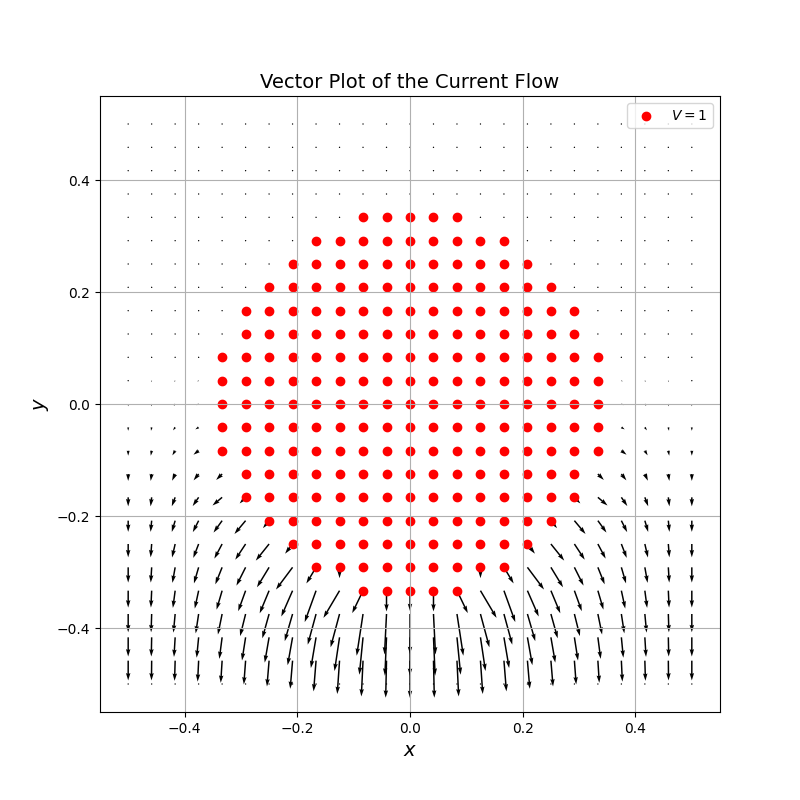
\includegraphics[scale=0.5]{10.png}
\end{figure}



\section{Conclusion}
The Laplace Equation has been solved using discrete differentiation iteratively.
This method of solving the Laplace Equation is generally not recommended.
This is because of the very slow coefficient with which the error reduces.



\end{document}
